% Springer LLNCS format conversion
\documentclass[runningheads]{llncs}

\usepackage[T1]{fontenc}

\usepackage{booktabs}
\usepackage{placeins}
\usepackage{float}
\usepackage{graphicx}
\usepackage{amsmath,amssymb,amsfonts}
\usepackage{algorithmic}
\usepackage{textcomp}
\usepackage{xcolor}
\usepackage{tikz}
\usepackage{scalerel}
\usepackage{orcidlink}
\usepackage{hyperref}
\usepackage{cite}

\usetikzlibrary{positioning}
\usetikzlibrary{svg.path}

\begin{document}

\title{Multimodal Sign Language Model}

\author{Christian Velasquez Borasino\orcidlink{0009-0004-6341-6924} \and \\
Giorgio Mancusi Barreda\orcidlink{0009-0001-7757-5262} \and
Rody Vilchez Marin\orcidlink{0009-0006-3773-9943}}

\institute{Universidad Peruana de Ciencias Aplicadas (UPC), Lima, Perú}

\titlerunning{Multimodal Sign Language Model}
\authorrunning{Borasino, Mancusi, and Vilchez}

\maketitle 

\begin{abstract}
Sign language translation (SLT) plays a key role in improving accessibility for deaf communities, but faces major challenges such as limited parallel video-text data. In this work, we present Imitator, an architecture that learns to produce text embeddings that align with those of a pretrained large language model (LLM), such as LLaMA. Our approach combines lightweight 1D convolutions and a transformer encoder with a cross-attention mechanism using learnable token queries to flexibly map variable-length video sequences into fixed-length text representations. The preliminary results show promising alignment metrics, suggesting the potential of this imitation-based strategy for SLT. Imitator model achieves a mean squared error with cosine similarity (MSE + Cossim) of $8 \times 10^{-4}$ on the validation set. These results highlight the potential of imitation-based embedding alignment as a lightweight alternative for sign language translation in low-resource contexts.


\end{abstract}

\keywords{Sign language \and embeddings \and distillation \and LSP}

\section{Introduction}

Sign language is the main mode of communication and expression for people who are deaf or hard of hearing \cite{ronchetti2023lsa}. Despite its importance, a significant communication gap persists between sign language users and non-users \cite{ojyyys_2022}, further exacerbated by the lack of accessible technological tools specifically designed for this population. Bridging this gap requires the development of effective translation systems capable of interpreting sign language accurately and robustly \cite{liu2024scopesignlanguagecontextual}.

Sign language consists of a wide variety of complex hand movements, facial expressions, and body gestures, making automatic translation a highly challenging task \cite{li2023adtrvlp}. One of the major obstacles for Peruvian Sign Language (LSP, lengua de señas peruana) translation is the scarcity of large-scale datasets containing parallel sign videos and textual annotations \cite{ojyyys_2022}. This data limitation makes it difficult to train end-to-end models, which often rely on direct mapping from sign-language input to textual output \cite{ronchetti2023lsa}.

Traditional SLT approaches typically involve predicting intermediate gloss sequences as a surrogate representation before generating text \cite{liu2024scopesignlanguagecontextual}. However, these models tend to suffer from limited accuracy and poor generalization, especially in low-resource settings \cite{li2023adtrvlp}. Recent studies confirm that even state-of-the-art gloss-based methods still outperform direct gloss-free approaches, although the gap is slowly narrowing thanks to advances in pretraining and contrastive learning \cite{zhao2024llavaSLT, li2023adtrvlp}.

In this work, we propose \textit{Imitator}, an architecture that learns to imitate the text representations of a large language model (LLM) such as LLaMA \cite{jaegle2021perceiver}, bypassing the need for intermediate gloss labels while maintaining semantic alignment with the target text.

\section{Related Work}

Liu et al.~\cite{liu2024scopesignlanguagecontextual} present SCOPE, a context-oriented framework for sign language recognition (SLR) and translation (SLT) tasks. This approach employs a multimodal encoder that integrates keypoints with textual embeddings extracted from a large language model (LLM). For translation, the language model is fine-tuned using prior conversational information. The authors also introduce a new dataset containing 72 hours of Chinese Sign Language videos in dialog contexts. SCOPE outperforms previous models on the PHOENIX-2014T and CSL-Daily benchmarks, demonstrating significant improvements in context-aware text generation.

Huang et al.~\cite{liu2024scopesignlanguagecontextual} propose SignCL, a contrastive learning framework for gloss-free SLT. Its objective is to reduce the performance gap between gloss-free and gloss-based methods by enforcing alignment between visual features and target text embeddings through contrastive loss. Despite these advances, gloss-based models still outperform SignCL on datasets such as CSL-Daily and RWTH-PHOENIX-Weather.

Li et al.~\cite{li2023adtrvlp} introduce ADTR-VLP, a pretraining framework for gloss-free SLT that combines visual–language contrastive objectives with a masked modeling task. This method achieves competitive performance with fewer parameters and narrows the performance gap with gloss-based approaches. However, the translation quality remains below that of fully supervised gloss-based systems.

Zhao et al.~\cite{zhao2024llavaSLT} extend LLaVA to the sign language domain by leveraging a vision–language model pretrained on sign videos and aligning visual inputs with LLM text embeddings. This approach further reduces the gap between gloss-based and gloss-free systems, demonstrating that large multimodal models can be adapted to sign language without explicit gloss supervision.

Taken together, these works illustrate a clear shift toward gloss-free translation by leveraging contrastive objectives, masked modeling, and multimodal alignment with large language models. Nevertheless, most existing approaches still depend on expensive pretraining or limited datasets, leaving an open opportunity for lightweight architectures capable of directly aligning visual inputs with LLM latent spaces. Our work addresses this gap by imitating LLM embeddings without gloss supervision, improving portability and reducing annotation costs.


\section{Methodology}

\begin{figure*}[htbp]
  \centering
  \includegraphics[width=0.8\textwidth]{15/figures/15_ImitatorArch.png}
  \caption{High-level architecture of the Imitator model including feature extraction, temporal encoding, and embedding alignment with LLaMA.}
  \label{fig:imitator-arch}
\end{figure*}

\subsection{The Imitator architecture}
The Imitator architecture is designed to map sequences of human keypoints into fixed-length text embeddings that align with a target language model (e.g., LLaMA), as illustrated in Fig.~\ref{fig:imitator-arch}. The model receives a temporal sequence of 2D skeleton keypoints per video frame and encodes them into compact embeddings through a convolutional-attentive pipeline, mixing convolutional networks and transformers.

\textbf{Feature projection}.A multi-layer perceptron (MLP) performs per-frame feature extraction by projecting the input from dimension \(D\) to the hidden size \(H=512\), then compressing it to \(H/2\). Each linear projection is followed by GELU activation and LayerNorm.

\textbf{Temporal modeling.} The reduced features are passed through a lightweight temporal encoder composed of two 1D convolutions. The first convolution (kernel size = 3, stride = 1, padding = 1) extracts local temporal features, while the second (kernel size = 1) performs channel mixing. Each stage uses LayerNorm and GELU activations. Finally, a linear projection maps the temporal output to the transformer hidden dimension \(hidden=512\).
  
An \emph{adaptive average pooling} layer is applied to reduce the temporal dimension from $T$ to $T'$ (set by default to $T' = 2L$), while the frame-level padding mask is propagated through \emph{adaptive max pooling} over the inverted validity map (\texttt{True}=pad, \texttt{False}=valid). A safeguard ensures that each batch retains at least one valid bin, preventing empty pooled sequences before entering the Transformer encoder.

\textbf{Rotary Positional Embeddings (RoPE)}
Instead of the classical sinusoidal positional encoding proposed by\cite{vaswani2023attentionneed}, we adopt rotary positional embeddings (RoPE) \cite{su2023roformerenhancedtransformerrotary} as a mechanism to encode temporal information. Unlike fixed absolute encodings, RoPE incorporates the position via learned rotations in the embedding space, allowing the model to reason directly over relative distances between tokens. This is particularly beneficial for sign language, which exhibits natural cyclic or repetitive patterns at both the word and sentence level. Moreover, RoPE encodes positional noise, such as jitter in keypoint detection, as small, smooth rotations in the query and key vectors, leading to stable attention weights and improved robustness to temporal variation.
In this work, we implement a RoPE transformer encoder modifying current implementation of transformer encoder layer by PyTorch. Our implementation is based on the modification of a \texttt{multi\_head\_attention\_forward} function to implement a RoPE operation into a MultiHeadAttention module.
    
To capture long-range dependencies across frames, we employ a transformer encoder with rotary positional embeddings (RoPE), as previously described. The encoder consists of \(n = 6\) layers, each with sixteen attention heads, GELU activations, and dropout rate of 0.2. Layer normalization is applied in pre-norm. The PyTorch transformer encoder layer was re-implemented to include a new argument, \texttt{use\_rotary=True}, enabling RoPE with a default base of \texttt{1000}.

\textbf{Projection to embedding space.} 
Each time step is independently projected into a target output space of dimension 3072. 
We selected an output dimensionality of 3072 to exactly match the token embedding width of the LLaMA-3.2B model. 
This ensures one-to-one compatibility between the visual representation and the latent text space of the LLM, enabling direct cosine-based supervision without additional projection layers. 
Target embeddings are obtained by passing the tokenized transcript through the LLaMA embedding layer, using Hugging Face's \texttt{Transformers} library to extract the embeddings corresponding to each input token. 
The resulting tensor \([B,\, T',\, \mathtt{output\_dim}]\) is interpreted as a set of visual keys and values. 

In all experiments, the transformer encoder employs a hidden size of \(H=512\), a feed-forward dimension of 2816, six layers (\(n=6\)), and sixteen attention heads (\(h=16\)). 
Both the encoder and cross-attention modules apply a dropout rate of 0.2. 
The convolutional front-end uses 256 channels, and the model outputs are $\ell_2$-normalized along the embedding dimension before loss computation to ensure stable cosine-based supervision.

\textbf{Cross-attention head.}Motivated by the need to align video sequences with textual outputs of up to 128 tokens the maximum number of tokens observed after tokenizing the transcript using the LLaMA model's tokenizer we define a fixed set of \(L = 128\) learnable token queries with positional encoding to ensure that the tokens remain distinguishable based on the temporal dimension of the video. 

Besides temporal modeling on the video stream, we assign each output query a learnable token-wise positional identity (\text{token\_posenc}). Specifically, for the $i$-th pseudo-token we form $Q_i = q_i + p_i$, where $p_i \in \mathbb{R}^d$ is a learned embedding that indexes the output slot, no video time. 

These act as latent slots, each extracting semantically meaningful information from the variable-length visual input via multi-head cross-attention. Each query \(Q \in \mathbb{R}^{B \times L \times d}\) attends over the frame-level representations \(M \in \mathbb{R}^{B \times T \times d}\), using sixteen attention heads and a dropout rate of 0.2. This mechanism enables the model to flexibly pool visual information into a structured output space of fixed length, suitable for alignment with language model embeddings.

The cross-attention block outputs a structured sequence of token-level embeddings rather than a single global vector. Each learnable query acts as a pseudo-token that aggregates information from different temporal regions of the video, analogous to language tokens in a sentence. During training, these query outputs are aligned position-wise with the corresponding LLaMA token embeddings. In downstream applications, the entire set of 128 aligned vectors can be averaged or pooled to form a global representation when required.


At runtime we select $T_q = \min(L, T')$ output queries, where $T'$ is the number of pooled frame-level representations. The learnable positional embeddings (\texttt{token\_posenc}) are added to the first $T_q$ query vectors to maintain token-wise distinctness. Each query $Q \in \mathbb{R}^{B \times L \times d}$ attends over the frame-level representations $M \in \mathbb{R}^{B \times T' \times d}$ using sixteen attention heads and a dropout rate of 0.2. This mechanism enables the model to flexibly pool visual information into a structured output space of fixed length, suitable for alignment with language model embeddings.

Inspired by the latent update mechanism of Perceiver IO~\cite{jaegle2021perceiver}, we apply a single cross-attention update, where the attended output is added residually to the input queries and then normalized:
\[
    X = \mathrm{LayerNorm}(Q + \mathrm{MultiHeadAttn}(Q, M, M)).
\]

To enhance representational capacity and training stability, the result is further processed 
by a residual feed-forward block composed of two linear layers (with an expansion factor of 2), 
GELU activation, and dropout of~0.1---analogous to the latent update step described 
in Perceiver~IO.

\subsection{Loss Function}

To train the Imitator model, we employ a masked loss that combines a mean squared error (MSE) term and a cosine similarity term, encouraging alignment between the predicted token embeddings and the corresponding target embeddings produced by a frozen language model. The loss is computed at the token level, aligning each of the $L$ predicted visual token embeddings with their textual counterparts from the LLaMA model. 

All predicted embeddings $\hat{E}$ are $\ell_2$-normalized before loss computation to stabilize magnitude differences across batches. Target embeddings $E$ are normalized within the cosine term. The dynamic scaling factor $\beta$ is detached from the gradient graph to prevent backpropagation through its computation, improving stability.

A binary mask is used to ignore padding tokens in shorter sequences. Specifically, given predicted embeddings $\hat{E} \in \mathbb{R}^{B \times L \times d}$ and target embeddings $E \in \mathbb{R}^{B \times L \times d}$, we first truncate both to the shortest common length ($L^\star$)
 to prevent shape mismatches. Let $v \in \{0,1\}^{B \times L^\star}$ denote the validity mask, where $v_{b\ell} = 1$ for valid tokens and $v_{b\ell} = 0$ for padding.

The masked mean squared error term is defined as:
\[
\mathcal{L}_{\text{MSE}} =
\frac{1}{\sum_{b=1}^{B}\sum_{\ell=1}^{L^\star} v_{b\ell}}
\sum_{b=1}^{B}\sum_{\ell=1}^{L^\star}
v_{b\ell} \cdot
\frac{1}{d}\left\| \hat{E}_{b\ell} - E_{b\ell} \right\|_2^2.
\]

Similarly, the masked cosine similarity loss is computed as:
\[
\mathcal{L}_{\text{cos}} =
\frac{1}{\sum_{b=1}^{B}\sum_{\ell=1}^{L^\star} v_{b\ell}}
\sum_{b=1}^{B}\sum_{\ell=1}^{L^\star}
v_{b\ell} \cdot
\left( 1 -
\frac{\hat{E}_{b\ell}}{\|\hat{E}_{b\ell}\|_2}
\cdot
\frac{E_{b\ell}}{\|E_{b\ell}\|_2} \right).
\]

To balance the two objectives, we introduce a dynamic scaling factor:
\[
\beta =
\frac{\mathcal{L}_{\text{MSE}}}{\mathcal{L}_{\text{cos}} + \varepsilon},
\quad \text{where } \varepsilon = 10^{-6}.
\]
Gradients are not propagated through $\beta$.

The final total loss is given by:
\[
\mathcal{L}_{\text{total}} = 
\mathcal{L}_{\text{MSE}} + 
\beta \, \mathcal{L}_{\text{cos}}.
\]

This formulation ensures that the model focuses exclusively on semantically valid tokens while dynamically adjusting the contribution of cosine similarity based on the relative magnitudes of the two losses. It thus enables stable and robust training even when sequence lengths and embedding magnitudes vary across samples. Importantly, the loss values are computed per token, reflecting the mean squared error over an embedding dimension of 3072.


This setup allows for robust learning even when the target embedding lengths vary across samples.

\begin{figure}
    \centering
    \includegraphics[width=1\textwidth]{15/figures/15_LossFunction.jpeg}
    \caption{Imitator Loss function}
    \label{fig:MSE}
\end{figure}

\subsection{Optimization schedule}

We adopt a learning rate schedule based on a linear warm-up followed by cosine decay, a strategy shown to stabilize training and improve generalization in transformer-based models \cite{vaswani2023attentionneed, loshchilov2017sgdr}. Specifically, the learning rate \(\eta_t\) at step \(t\) is defined by:

\[
\eta_t = 
\begin{cases}
\frac{t}{T_w}, & \text{if } t < T_w \\
\frac{1}{2} \left(1 + \cos\left( \pi \cdot \frac{t - T_w}{T - T_w} \right) \right), & \text{otherwise}
\end{cases}
\]

where \(T_w\) is the number of warm-up steps (typically 5 epochs), and \(T\) is the total number of training steps. The scheduler is implemented via PyTorch’s \texttt{LambdaLR}, which dynamically adjusts the learning rate each step. This approach allows the optimizer to ramp up gradually at the start, avoiding instability, and then anneal smoothly to improve convergence as training progresses.

\subsection{Data Preprocessing and Preparation}

\subsubsection{Video Selection}
To improve data quality, we excluded videos whose labels contained special characters (such as symbols). After filtering, a total of 4{,}100 videos were retained for training and validation.

\subsubsection{Keypoint Extraction}
To obtain a standardized representation across all sign language videos, we used the RTMPose-L model from the RTMlib repository \cite{rtmlib}. This model extracts 133 keypoints per frame, including body, hand, and facial landmarks. This 2D representation captures the spatial complexity of sign language gestures while remaining compact enough for efficient processing. All videos were processed at 30 fps, and keypoints were extracted at the original video resolution.

\subsubsection{Removed Extra Keypoints}
To reduce unnecessary keypoints, such as those corresponding to legs and face border, we decreased the total number from 133 to 89. As shown below, some of the removed keypoints include those on the legs and along the face border.

\subsubsection{Normalization and Padding Handling}
To standardize spatial scale and position, keypoints are normalized using a shoulder-centered coordinate system. The skeleton is centered at the midpoint between the shoulders and scaled by the shoulder distance. Keypoints with null coordinates (e.g., (0,0)) are masked and replaced with out-of-range values (e.g., (-3,-3)), preserving their presence without affecting model training.


\begin{figure}
    \centering
    \includegraphics[width=0.5\textwidth]{15/figures/15_SignerKeypointsExample.jpeg}
    \caption{Signer Keypoints}
    \label{fig:keypoints}
\end{figure}

\subsubsection{Embedding Generation and Target Construction}
For each video, we generate a fixed-size (3072-dimensional) textual embedding using the LLaMA-3.2B model. These embeddings serve as soft targets during training, enabling alignment in shared embeddin space without the need for gloss annotations.

 Unlike methods such as SignCL or LLaVA-SLT, our architecture does not depend on retraining the LLM when it is updated. Imitator remains compatible as long as embedding space itself is unchanged. This design allows the learned embeddings to be directly indexed within the LLM's latent space, thereby eliminating retraining costs and enhancing portability across models.

\subsubsection{HDF5 Storage Format}
All preprocessed data (keypoints, embeddings, labels) are stored in HDF5 format using a hierarchical structure. This format supports modular dataset access, fast loading, and version control. Each dataset is organized into separate groups, enabling selective activation during training or ablation studies.

\subsection{Data loading and sampling}

An overview of the full data flow—from keypoint input to embedding alignment—is shown in Fig.~\ref{fig:architecture}. This diagram summarizes how each component processes the input to produce LLM-aligned embeddings.

\begin{figure}[ht]
\centering
\resizebox{\columnwidth}{!}{%
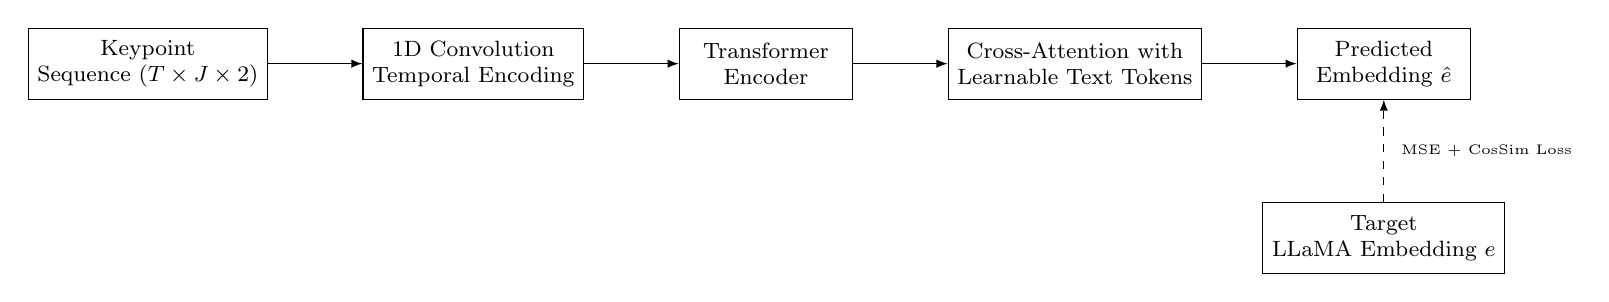
\begin{tikzpicture}[node distance=0.8cm and 1.2cm, every node/.style={font=\footnotesize}, >=latex]

\node (input) [draw, minimum width=2.2cm, minimum height=0.9cm, align=center] {Keypoint \\ Sequence $(T \times J \times 2)$};
\node (conv) [draw, right=of input, minimum width=2.2cm, minimum height=0.9cm, align=center] {1D Convolution \\ Temporal Encoding};
\node (transformer) [draw, right=of conv, minimum width=2.2cm, minimum height=0.9cm, align=center] {Transformer \\ Encoder};
\node (crossatt) [draw, right=of transformer, minimum width=2.6cm, minimum height=0.9cm, align=center] {Cross-Attention with \\ Learnable Text Tokens};
\node (output) [draw, right=of crossatt, minimum width=2.2cm, minimum height=0.9cm, align=center] {Predicted \\ Embedding $\hat{e}$};
\node (target) [below=1.3cm of output, draw, minimum width=2.2cm, minimum height=0.9cm, align=center] {Target \\ LLaMA Embedding $e$};

\draw[->] (input) -- (conv);
\draw[->] (conv) -- (transformer);
\draw[->] (transformer) -- (crossatt);
\draw[->] (crossatt) -- (output);
\draw[->, dashed] (target) -- (output) node[midway, right, xshift=0.1cm] {\tiny MSE + CosSim Loss};

\end{tikzpicture}
}
\caption{Overview of the Imitator architecture. The input sequence of keypoints is processed via 1D convolutions and a transformer encoder. A cross-attention module with learnable text tokens maps the temporal features to a fixed-dimensional embedding aligned with the LLaMA target.}
\label{fig:architecture}
\end{figure}

\section{Dataset and Experimental Setup}

\subsection{Datasets}

\subsubsection{LSA64}
We evaluate our framework on LSA64~\cite{Ronchetti2016}, an isolated Argentinian Sign Language dataset containing 3,200 video recordings of 64 lexical signs performed by 10 subjects (five repetitions per sign) under controlled conditions, with signers wearing colored gloves to facilitate hand tracking. Each sample consists of an RGB video sequence, from which we extract 2D keypoints using an off-the-shelf pose estimator. Our pipeline does not employ gloss annotations.

\subsubsection{Peruvian Sign Language (LSP) PUCP-DGI156}
We further leverage the PUCP-DGI156 dataset~\cite{ojyyys_2022}, which offers original and sign-segmented MP4 videos, SRT subtitle files, and MediaPipe-based pose estimations (27 keypoints) of continuous Peruvian Sign Language. The dataset includes over 1 GB of segmented footage and 690 MB of pose data, segmented using ELAN software.

\subsubsection{Peruvian Sign Language (LSP) PUCP 305}
We further utilize the PUCP 305 dataset~\cite{JU4OLG_2024}, which provides original and sign-segmented MP4 videos of continuous Peruvian Sign Language. The dataset comprises over 2 GB of video material, containing 526 recordings featuring various signers and signs.

\noindent  Although the primary training data originate from the Argentinian Sign Language (LSA), its structural and visual properties differ markedly from those of the Peruvian Sign Language (LSP), including differences in vocabulary, grammatical organization, and signer-specific conventions \cite{ronchetti2023lsa, ojyyys_2022}. Such divergence introduces a cross-linguistic domain shift that provides a suitable scenario to evaluate the robustness and generalization capacity of the proposed gloss-free embedding model. To explicitly incorporate this variability into the learning process, both LSA and LSP datasets are merged prior to applying the data-splitting procedure detailed in Section~\ref{sec:data-splits}.

\subsection{Data Splits}\label{sec:data-splits}
All samples from the combined datasets are randomly shuffled without consideration of signer identity or gloss annotation. The partitioning is performed at the sample (video-fragment) level rather than by signer or gloss, yielding 3,280 samples (80\%) for training and 820 samples (20\%) for validation.The adopted intrasigner setting allows the same signer to appear in both partitions, which is consistent with our objective of assessing generalization across instances rather than across unseen signers. At this stage, no separate test set is defined; all quantitative evaluations are conducted on the validation set, as the present work constitutes an initial exploration of the proposed approach under cross-linguistic variability.

\subsection{Cross validation}
\label{sec:cross-validation}
We employ a 5-fold cross-validation protocol to improve robustness and reduce variance in reported metrics. All datasets are merged and randomly shuffled at the sample level, disregarding gloss and signer identity. In each fold, 80\% of samples are allocated for training and 20\% for validation. The reported metrics correspond to the average performance across all five folds. Note that this protocol is intra-signer: the same signer may appear in both splits. A held-out test set is not defined at this stage.

\begin{table}[H]
\centering
\caption{Training and validation losses per fold under the 5-fold cross-validation protocol (intra-signer). Mean and standard deviation (std) are reported across folds.}
\label{tab:cv-loss}
\setlength{\tabcolsep}{8pt}
\begin{tabular}{lcc}
\hline
\textbf{Fold} & \textbf{Train Loss} & \textbf{Val Loss} \\
\hline
1 & 6.44e$^{-4}$ & 8.04e$^{-4}$ \\
2 & 8.51e$^{-4}$ & 8.16e$^{-4}$ \\
3 & 6.53e$^{-4}$ & 8.06e$^{-4}$ \\
4 & 6.30e$^{-4}$ & 8.10e$^{-4}$ \\
5 & 6.42e$^{-4}$ & 7.71e$^{-4}$ \\
\hline
\textbf{Average} & \textbf{6.84e$^{-4}$} & \textbf{8.01e$^{-4}$} \\
\textbf{Std} & \textbf{9.37e$^{-5}$} & \textbf{1.76e$^{-5}$} \\
\hline
\end{tabular}
\end{table}

The detailed results for each fold are summarized in Table~\ref{tab:cv-loss}. 
We observe very low variability across folds: the training loss averages $6.84\times10^{-4}$ with a standard deviation of $0.0005$, while the validation loss remains consistently around $8.04\times10^{-4}$. 
This stability indicates robust training dynamics and consistent embedding alignment performance under the proposed cross-validation protocol.
Importantly, these loss values are computed per token, reflecting the mean squared error over an embedding dimension of 3072.

\subsection{Training Scheme}
The model was trained for 100 epochs using the AdamW optimizer with a base batch size of 64. Gradient accumulation across two mini-batches was employed, resulting in an effective batch size of 128 samples per optimization step. A linear warm-up followed by cosine decay was applied as the learning rate schedule. Training was performed on an NVIDIA L4 GPU with 24 GB of VRAM and required approximately 1 hour to complete due to early stopping being enabled. The dataset was split into 80\% for training and 20\% for validation  with cross-validation. Without signer-exclusive evaluation was conducted at this stage.

\subsection{Model Metrics}  
Most of our training videos contain short utterances of only one to three words. In this regime, the visual evidence for each word spans a large portion of the sequence, which naturally yields high attention entropy: the cross-attention module behaves as a form of soft temporal pooling rather than a precise frame locator. This behavior is desirable—it prevents overfitting to a few frames and promotes robustness to signer speed variations, coarticulation, and pose-detection jitter.
Based on the images below shows the model alignment and the Cross-Attention Map. 

\begin{figure}[!htbp]
  \centering
  \includegraphics[width=\linewidth]{15/figures/15_AlignmentMetrics.jpeg}
  \caption{Alignment metrics across training epochs.}
  \label{fig:alignment-metrics}
\end{figure}
\FloatBarrier
The retrieval metrics (R@K) show a consistent improvement across epochs in both directions (video$\rightarrow$text and text$\rightarrow$video), approaching near-perfect alignment at higher K values. 
This suggests that the model progressively learns a shared embedding space where corresponding video and text samples become close neighbors.
In the geometric metrics, the alignment MSE decreases while CKA remains high and the procrustes error declines slightly, confirming better structural correspondence between the two modalities. 
Uniformity values for both visual and textual embeddings remain stable, suggesting that the model maintains a good distributional spread and avoids representation collapse.

\paragraph{Linguistic Evaluation.}
Although the current experiments focus on short utterances (one to three words), we also report a preliminary linguistic metric using BLEU scores computed with the \texttt{NLTK} implementation.
Since most clips contain a single lexical item, BLEU-1 (unigram precision) provides the most meaningful signal, while higher-order scores (BLEU-2 and BLEU-4) naturally approach zero due to the absence of multi-word n-grams.
Table~\ref{tab:bleu} summarizes the results across three datasets: \textbf{Dataset~1} (LSA64) and \textbf{Datasets~3} and \textbf{5} (LSP).
All values are reported on a corpus level. BLEU-1 for LSA64 reaches $0.5975$ ($59.8\%$), indicating that the model correctly associates approximately six out of ten visual tokens with their textual counterparts.
Lower values on LSP (0.0244 and 0.0158) reflect the greater variability, signer diversity, and overall noise of that corpus.
Because the evaluation clips contain isolated signs, these BLEU values should be interpreted as a proxy for word-level retrieval accuracy rather than full-sentence translation quality.

\noindent These results confirm that the model maintains consistent visual–textual associations even under a strictly gloss-free training regime. Here, BLEU-1 serves as a complementary measure to retrieval and alignment metrics, capturing the correctness of the lexical-level mapping learned by the model.

\begin{table}[t]
\centering
\caption{Corpus-level BLEU scores for one-word evaluation clips.}
\label{tab:bleu}
\begin{tabular}{lccc}
\toprule
\textbf{Dataset} & \textbf{BLEU-1} & \textbf{BLEU-2} & \textbf{BLEU-4}\\
\midrule
Dataset 1 (LSA64) & 0.5975 & 0.1543 & 0.0091\\
Dataset 3 (LSP)   & 0.0244 & 0.0079 & 0.0046\\
Dataset 5 (LSP)   & 0.0158 & 0.0020 & 0.0007\\
\bottomrule
\end{tabular}
\end{table}

\FloatBarrier
\noindent These results confirm that the model maintains consistent visual–textual associations even under a strictly gloss-free training regime. Here, BLEU-1 serves as a complementary measure to retrieval and alignment metrics, capturing the correctness of the lexical-level mapping learned by the model.

\begin{figure}[!htbp]
    \centering
    \includegraphics[width=0.75\textwidth]{15/figures/15_Cross-Attention}
    \caption{Cross-attention visualization at epoch 45.}
    \label{fig:CrossAttention}
\end{figure}

The cross-attention map at epoch 45 reveals moderately structured token–frame associations, with a positive correlation ($\rho = 0.77$) between token index and attended frame position.
The attention weights remain broadly distributed ($\mathcal{H} = 1.0$) and cover approximately $3.4\%$ of the total frame area, indicating that each token attends to multiple temporal regions rather than isolated moments.
Given that the videos are short (1–3 words per clip), this broad attention is expected and reflects the compact temporal nature of the input rather than a failure of alignment.

\section{Results}

Under the 5-fold cross-validation protocol (Sec.~\ref{sec:cross-validation}), the Imitator model achieved an average validation loss of \(8.01 \times 10^{-4}\) and an average training loss of \(6.84 \times 10^{-4}\) (Table~\ref{tab:cv-loss}). 
These results are consistent with the single hold-out evaluation, where the model obtained a mean squared error with cosine similarity (MSE + Cossim) of approximately \(8 \times 10^{-4}\) on the validation set. 
This metric was computed between the predicted embedding, \(\hat{e}\), and the target embedding, \(e\), generated by the LLM. 

Across all five folds, the model exhibited minimal variance, with training losses ranging from \(6.30 \times 10^{-4}\) to \(8.51 \times 10^{-4}\), and validation losses remaining stable around \(8.0 \times 10^{-4}\). 

This consistency indicates robust convergence and suggests that the alignment mechanism generalizes effectively across different data partitions.

\section{Discussion}

The results confirm that Imitator is capable of extracting semantically meaningful representations from 2D keypoint sequences and aligning them with textual embeddings from a large language model. This demonstrates that rich linguistic information can be inferred directly from body motion, even in the absence of gloss annotations.

While the performance is encouraging, we acknowledge several limitations. First, the validation set may be overly optimistic due to the presence of the same signers in both training and validation (intrasigner overlap). Second, our results may reflect constraints imposed by consumer-grade hardware, such as suboptimal keypoint quality or limited batch sizes during training. Third, the dataset is derived from a single domain (news broadcast), which may affect generalization.

\section{Conclusions and Future Work}

\subsection{Summary of Findings}

In this work, we introduced Imitator, a novel sign language model that aligns sequences of 2D keypoints with text embeddings from a pretrained large language model (LLM) without relying on intermediate gloss annotations. The proposed architecture combines lightweight convolutional layers, transformer encoders, and a cross-attention mechanism with learnable token queries to encode complex spatio-temporal dynamics of sign language into fixed-dimensional representations. By enabling direct supervision at the embedding level, Imitator facilitates faster adaptation to different sign languages or updated LLM backbones without requiring model retraining. Experimental results demonstrate that the model achieves high alignment accuracy using only motion-based inputs, validating the potential of gloss-free sign language translation in low-resource scenarios.
\subsection{Extended Discussion and Future Directions}

Imitator's alignment mechanism provides a promising foundation for low-cost and flexible sign language understanding systems. Unlike methods that require expensive retraining or fine-tuning of large language models, our approach aligns directly with the target embedding space, which improves adaptability to changes in the language model backend and reduces maintenance costs.

Despite the encouraging results, several avenues remain open for future exploration. A key challenge lies in improving generalization, particularly by evaluating signer-independent scenarios and cross-dataset transfer to mitigate potential overfitting to the current corpus. Another critical aspect is downstream integration: assessing how the learned embeddings perform in tasks such as retrieval, classification, or LLM prompting, especially in multilingual or assistive contexts.

Further work is needed in visualization and explainability, where tools for analyzing embedding trajectories, token attention distributions, and interpretability maps could offer deeper insights into model behavior. From a benchmarking perspective, incorporating established gloss-free SLT baselines would contextualize the effectiveness of our imitation-based strategy and highlight its comparative advantages.

In terms of applications, Imitator’s lightweight design suggests potential for real-time deployment in sign recognition and communication assistance systems. External validation also remains an important milestone: Defining a held-out test set and evaluating performance on additional public benchmarks will be essential to confirm real-world applicability. Extending the model toward continuous SLT tasks, where sequence-level textual targets are required, represents another promising challenge.

Finally, exploring LLM agnosticism by adapting the framework to alternative models such as Gemma-3B could provide further evidence of portability across architectures. Complementarily, advanced data augmentation techniques — including generative motion synthesis, signer-style transfer, or learned spatio-temporal perturbations — may enhance robustness and performance in low-resource scenarios.

Our findings underscore the feasibility of gloss-free learning through embedding alignment with pretrained LLMs. As accessibility tools continue to evolve, models like Imitator have the potential to play a central role in making digital systems more inclusive for deaf communities worldwide.


\bibliographystyle{splncs04}
\bibliography{15/15}

\end{document}